\documentclass[aspectratio=169,xcolor=table]{beamer}
%aspcetratio >> 1610 169 149 54 43 32
%The themes:
%\usetheme[style=classic]{mharvellous}
\usetheme[style=dark]{mharvellous}
%\usetheme[style=mracula]{mharvellous}
%\usetheme[style=default]{mharvellous}
%*--------------------------------------------------
%\usepackage{helvet}
%*--------------------------------------------------
\usepackage{bibunits}  
%\setbeamertemplate{bibliography item}{[\theenumiv]}
\setbeamertemplate{bibliography item}{\insertbiblabel}
\defaultbibliography{bibliography}
%\defaultbibliographystyle{IEEEtran}
%\defaultbibliographystyle{amsalpha}
\defaultbibliographystyle{abntex2-alf}
%\bibliography{bibliography}
%\usepackage[backend=biber,style=alphabetic,citestyle=authoryear]{biblatex}
% \addbibresource{bibliography.bib}
%\usepackage{natbib}
\usepackage{bibentry}
%*--------------------------------------------------
\usepackage{lipsum}
\usepackage{epigraph}
\usepackage{graphicx}
\usepackage{multirow}
%\usepackage{enumitem}
\usepackage{array}
%\usepackage{multimedia}
\usepackage{media9}
%\usepackage{pdfpc-movie}
\usepackage{circledsteps}
\usepackage{listings}
\usepackage[normalem]{ulem}
%\usepackage{Sweave}
%\usepackage{xkeyval}
%\usepackage{palatino}
%\usepackage{pgfpages}
\usepackage{float}
%*--------------------------------------------------
\usepackage[timeinterval=1]{tdclock}
%\usepackage[font=Times,timeinterval=1, timeduration=200,resetatpages=all]{tdclock}
%\usepackage[font=Times,timeinterval=10, timeduration=2.0, timedeath=0, fillcolorwarningsecond=white!60!yellow,timewarningfirst=50,timewarningsecond=80,resetatpages=2]{tdclock}
%*--------------------------------------------------
\usepackage{url}
\usepackage{tabularx,booktabs}
\usepackage{threeparttable}
\usepackage[absolute, overlay]{textpos}
%*--------------------------------------------------
\usepackage{framed, color}
\usepackage[tikz]{bclogo}
\usepackage{spot}
\setspotlightcolor{red!50}
% %\setspotlightstyle{star, fill=red!50}
% %\setspotlightstyle{star points=7}
\usepackage{color,soul}
%\usepackage{xcolor}
\usepackage{tcolorbox}
\usepackage{xcolor}
\usepackage[export]{adjustbox}
\usepackage{verbatim}
\usetikzlibrary{trees,shapes,arrows}
\usepackage{fancyvrb}
\usepackage{float}
%*--------------------------------------------------
\usepackage{amsmath}
\usepackage{xfrac}
\usepackage{units}
\usepackage{ulem}
%*-------------------------------------------------------------------------------
%\newcolumntype{C}[1]{>{\centering\arraybackslash}m{#1}}
\newcolumntype{L}[1]{>{\raggedright\let\newline\\\arraybackslash\hspace{0pt}}m{#1}}
\newcolumntype{C}[1]{>{\centering\let\newline\\\arraybackslash\hspace{0pt}}m{#1}}
\newcolumntype{R}[1]{>{\raggedleft\let\newline\\\arraybackslash\hspace{0pt}}m{#1}}
%*-------------------------------------------------------------------------------
%\pgfpagesuselayout{2 on 1}[a4paper,border shrink=5mm]
%\setbeamertemplate{note page}[plain]
%\setbeameroption{show notes on second screen=bottom}
%*-------------------------------------------------------------------------------
\setbeameroption{hide notes}
%\setbeameroption{show only notes}
%\setbeameroption{show notes on second screen=right}
\setbeamertemplate{note page}{\pagecolor{yellow!5}\insertnote}
%*-------------------------------------------------------------------------------

%*-------------------------------------------------------------------------------
\title              {Horta-bot}
\subtitle           {sistema CNC para suporte as hortas caseiras.}
\author             {João Gabriel da Anunciação Calmon}
\email              {joao.calmon@aln.senaicimatec.edu.br}
\advisor            {Orientador: Marco A. dos Reis}
\institute          {Robótica e Sistemas Autônomos, Senai Cimatec}
\date               {Abril de 2022}
% \ulogo        		{Template/logosenaicimatecnegativo}
% \ulogof             {Template/logosenaicimatec2020}
% \ulogoo        		{Template/rosa-logo}
% \ulistelement    	{Template/bullet-white}

%*-------------------------------------------------------------------------------
\graphicspath{{Source/pictures/}}
%*-------------------------------------------------------------------------------
\totalNoSlidesDisabled % To turn off the total number of slides in the footer. Comment this if you want the total number of slides in the footer
%*-------------------------------------------------------------------------------
\begin{document}
%*----------- COVER -------------------------------------------------------------
 \begin{frame}[t,plain]
%*----------- sound--------------------------------
    \includemedia[
        %width=1ex,
        %height=1ex,
        %activate=pageopen, 
        activate=onclick,
        deactivate=onclick,
        %passcontext,
        transparent,
        addresource=./Source/sounds/hip-hop.mp3,
        flashvars={
                    source=./Source/sounds/hip-hop.mp3
                    %&autoPlay=true
                    &autoRewind=true
                    &Play=2s
                    &repeat=always
                    %&Loop=true
        }
    ]
    {}{VPlayer.swf}
%*----------- start-page--------------------------
    \titlepage
    %*----------- notes-------------------------------
    \note[item]{Notes can help you to remember important information. Turn on the notes option.}
\end{frame}
%-
%*----------- SECTIONS ----------------------------------------------------------
%*-----------ORIENTADOR -------------------------------------------------------------
\begin{frame}[t]{Horta-bot}
    \transboxout[duration=0.5]
    \framesubtitle{Marco A. Reis}
    \begin{columns}
        \column{.075\textwidth}
        \column{.4\textwidth}
            \includegraphics[width=.7\textwidth]{darwin-op}
        \column{.55\textwidth}
            \begin{itemize}
                \justifying
                \item Possui graduação em Engenharia Elétrica pela Universidade Federal do Paraná (1996) e mestrado em Engenharia de Produção pela Universidade Federal de Santa Catarina (2003);
                % \item 20 DoF\footnote{do inglês, graus de liberdade};
                \item (...);
            \end{itemize}
    \end{columns}
 %*----------- notes
    \note[item]{Notes can help you to remember important information. Turn on the notes option.}
\end{frame}
%-

%*----------- SLIDE -------------------------------------------------------------
\begin{frame}[t]{Justificativa} 
    \transdissolve[duration=0.5]
    %\newline
        \begin{columns}[t]
            \column{.05\linewidth}
            \column{.6\linewidth}
                \begin{itemize}
                    \justifying
                    \item A rotina da vida urbana torna o tempo um recurso escasso, dificultando atividades de cultivo; \cite{G1:3xtransito}
                    \item Há uma longa e complexa cadeia logística na disponibilização de alimentos orgânicos; \cite{silva:cadeiaprodutiva}
                    \item A busca por alimentos orgânicos tem crescido;  \cite{sebrae:organicos}.
                    \item O cultivo de pequenos temperos e hortaliças no ambiente domiciliar favorece uma cultura mais "verde" e participativa; \cite{G1:pequenoagricultor}
                \end{itemize}
            \column{.45\linewidth}
            \begin{center}
            %\centerline{
                \begin{figure}
                    %\includegraphics[width=1\textwidth]{pista}
                    % \caption{Pista de corrida}
                    \hspace{125pt}
                    \roundpic[xshift=0cm,yshift=0cm]{4cm}{5cm}{organic-icon.png}
                    %\caption{Pista de corrida \cite{agostini2007}}
                \end{figure}
            %}
            \end{center}
        \end{columns}
%*----------- notes
    \note[item]{Notes can help you to remember important information. Turn on the notes option.}
\end{frame}
%-

%*----------- SLIDE -------------------------------------------------------------
\begin{frame}
    %\transdissolve[duration=0.5]
    %\hspace*{-1cm}
    \begin{columns}
        %\column{.01\textwidth}
        \column{0.4\textwidth}
            ~\hfill
            \vbox{}\vskip-1.4ex%
            \begin{beamercolorbox}[sep=6em, colsep*=18pt, center, wd=\textwidth, ht=\paperheight]{title page header}%
                \begin{center}
                    \textbf{\huge{PROBLEMA}}\par
                    \vspace*{0.3cm}
                    \textbf{\huge{DE}}\par
                    \vspace*{0.3cm}
                    \textbf{\huge{PESQUISA}}
                \end{center}
            \end{beamercolorbox}%
        \hfill\hfill
        \column{.05\textwidth} 
        \column{.55\textwidth}
        \begin{center}
            \huge{\textbf{"De que forma é possível cultivar hortaliças orgânicas de forma autônoma no ambiente residencial dos centros urbanos?"}}
        \end{center}
        \hfill
       
    \end{columns}
  
 %*----------- notes__
    \note[item]{Notes can help you to remember important information. Turn on the notes option.}
\end{frame}
%-

%*----------- OBJETIVO GERAL -------------------------------------------------------------
\begin{frame}[c]{Objetivo Geral} 
    \transdissolve[duration=0.5]
   
    \begin{center}
        \Wider{%
        \begin{shaded}
        \begin{center}
            \vspace*{0.4cm}
            \resizebox{!}{1.3cm}{%
               % \color{bg} O objetivo é ter um objetivo.
                \begin{tabular}{ccc}
                    Desenvolver um sistema robótico capaz de realizar o \\
                    monitoramento de hortaliças e realizar a plantação\\ 
                    das mesmas.       
                  \end{tabular}
            }%
        \end{center}
        \end{shaded}
        }%
    \end{center}
    
   
%*----------- notes
    \note[item]{Notes can help you to remember important information. Turn on the notes option.}
\end{frame}
%-
%*----------- SLIDE -------------------------------------------------------------
\begin{frame}[t]{Objetivos Específicos}
    \transboxout[duration=0.5]
    \begin{columns}
        \column{.1\textwidth}
        \column{1.8\textwidth}
            \begin{enumerate}
                \item Realizar o estudo do estado da arte;
                \item Desenvolver sistema de movimentação para a unidade de supervisionamento;
                \item Desenvolver sistema de monitoramento visual (computacional);
                \item Desenvolver sistema de atuação para plantação e aquecimento;
                \item Desenvolver página de informações para o compartilhamento dos resultados com 
                \\ os usuários;
                \item Realizar demonstração do sistema;
                \item Desenvolvimento de artigos científicos.

            \end{enumerate}
    \end{columns}
 %*----------- notes
    \note[item]{Notes can help you to remember important information. Turn on the notes option.}
\end{frame}
%-

%*----------- SLIDE -------------------------------------------------------------
\begin{frame}[c]{Metodologia}
    %\transboxin[duration=1,direction=30]

    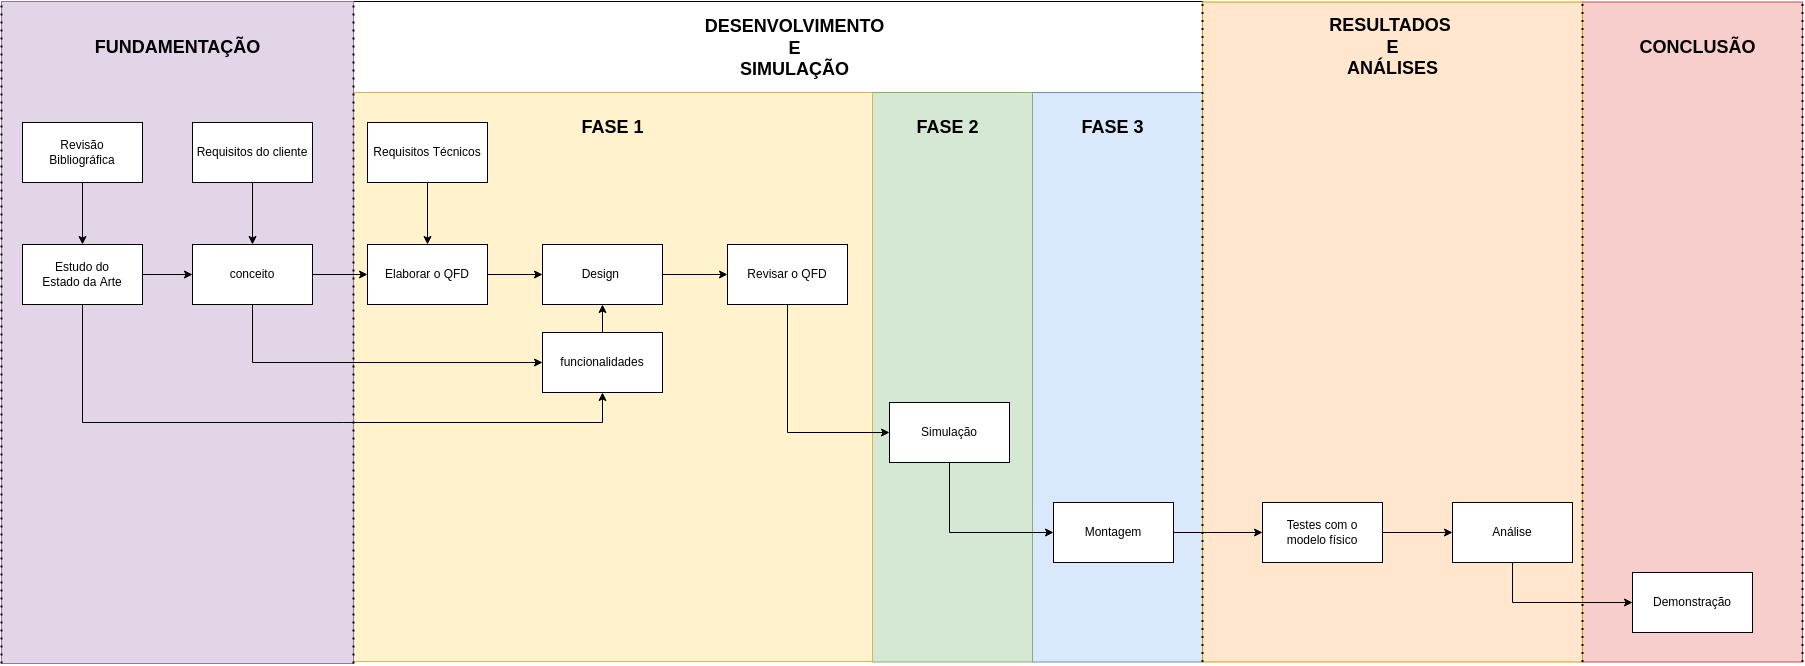
\includegraphics[width=1.04\textwidth]{metodologia.png}

%*----------- notes
    \note[item]{Notes can help you to remember important information. Turn on the notes option.}
\end{frame}
%-

%*----------- SLIDE -------------------------------------------------------------
\begin{frame}[c]{Método BiLi}
    %\transboxin[duration=1,direction=30]
    \begin{figure}
        \centering
        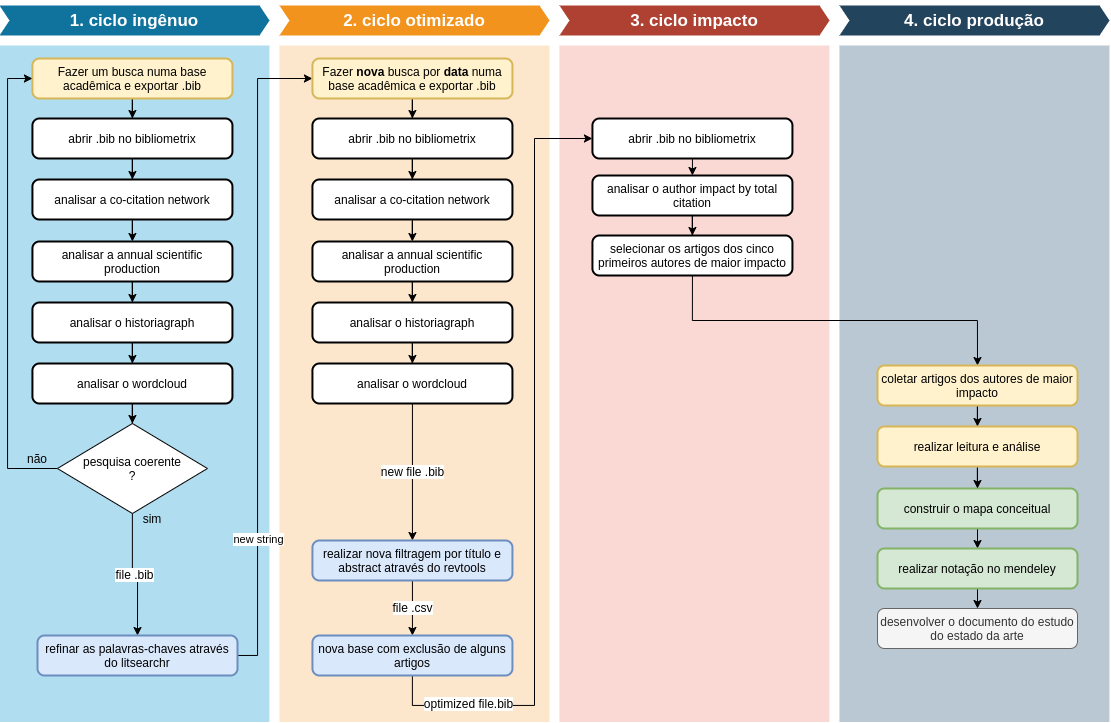
\includegraphics[width=0.7\textwidth]{bili-fluxograma.png}
    \end{figure}
%*----------- notes
    \note[item]{Notes can help you to remember important information. Turn on the notes option.}
\end{frame}
%-

%*----------- SLIDE -------------------------------------------------------------
\begin{frame}[c]{Mapa de Palavras}
    \framesubtitle{Ciclo Ingênuo X Ciclo Otimizado}
    %\transboxin[duration=1,direction=30]
    \begin{figure}
        \centering
        
\includegraphics[width=1\textwidth]{bili-wordclould.png}
    \end{figure}
%*----------- notes
    \note[item]{Notes can help you to remember important information. Turn on the notes option.}
\end{frame}
%-

%*----------- SLIDE -------------------------------------------------------------
\begin{frame}[c]{Evolução Temática}
    %\transboxin[duration=1,direction=30]
    O tema de pesquisa apresentou \textbf{crescimento anual} de produção científica de \textbf{10,76\%} (2016 - 2021)\\
    \begin{figure}
        \centering
        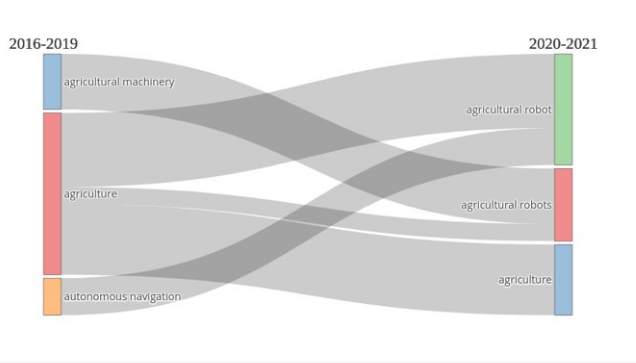
\includegraphics[width=0.65\textwidth]{bili-thematic-evolution.png}
    \end{figure}
%*----------- notes
    \note[item]{Notes can help you to remember important information. Turn on the notes option.}
\end{frame}
%-

%*----------- SLIDE -------------------------------------------------------------
\begin{frame}[c]{Referencial Teórico}
    
% table
%*----------- notes
    \note[item]{Notes can help you to remember important information. Turn on the notes option.}
\end{frame}
%-
%*----------- SLIDE -------------------------------------------------------------
\begin{frame}[c]{Roadmap}
    %\cutpic{0.30cm}{3cm}{element}
    \begin{tabular}{cccc}
        \rule{30pt}{0ex}  &   \href{https://element.io/}{
\includegraphics[width=.2\textwidth]{element-1.png}} & \rule{15pt}{0ex} 
\includegraphics[width=.15\textwidth]{notion.png} \rule{15pt}{0ex}& 
\includegraphics[width=.16\textwidth]{github.png}\\
    \end{tabular}

    \begin{tabular}{ccc}
        \phantom{This text s invisible} &   
\includegraphics[width=.2\textwidth]{trello.png} \rule{5pt}{0ex}& 
\includegraphics[width=.2\textwidth]{project-libre.png} \\
    \end{tabular}
%*----------- notes
    \note[item]{Notes can help you to remember important information. Turn on the notes option.}
\end{frame}
%-

% %*----------- SLIDE -------------------------------------------------------------
% \begin{frame}[c]{}
% \begin{figure}
%     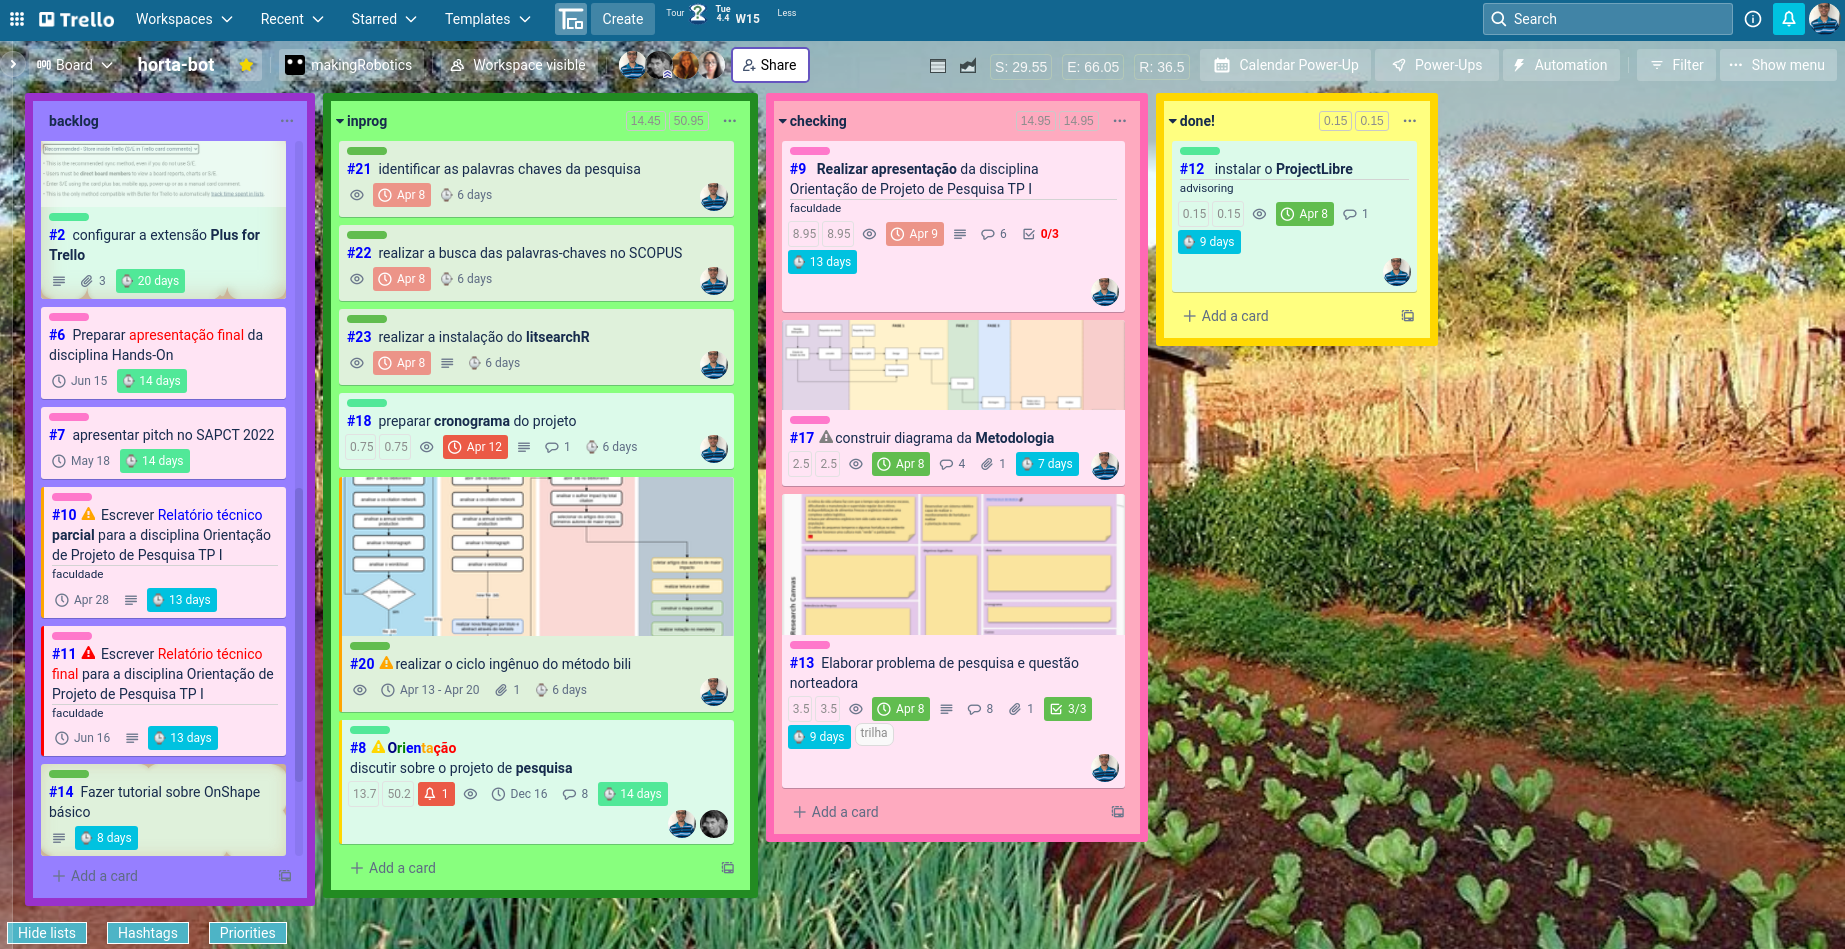
\includegraphics[width=1\textwidth]{trello-print.png}
% \end{figure}


% %*----------- notes
%     \note[item]{Notes can help you to remember important information. Turn on the notes option.}
% \end{frame}
% %-
%*----------- SLIDE -------------------------------------------------------------
\begin{frame}[t]{Resultado Esperado}
    \transboxout[duration=0.5]
    \vspace*{0.2cm}
    \begin{columns}
        \column{.1\textwidth}
        \column{1.8\textwidth}
                \Large{Uma horta automatizada cultivada, mantida e monitorada por um \\
                    sistema CNC \\
                     %\vspace*{\vertspaceresultado}
                }
    \end{columns}
    
    \vspace*{0.3cm}
    \begin{figure}
        
\includegraphics[width=.45\textwidth]{resultados.jpg}
    \end{figure}
 %*----------- notes
    \note[item]{Notes can help you to remember important information. Turn on the notes option.}
\end{frame}
%-

%*----------- SLIDE -------------------------------------------------------------
\begin{frame}[t]{Principais Aprendizados}
    \transboxout[duration=0.5]
    ipsum
 %*----------- notes
    \note[item]{Notes can help you to remember important information. Turn on the notes option.}
\end{frame}
%-
%----------------------------------------------------SLIDE------------------
 \begin{frame}[t, allowframebreaks]{Referências}
 %\frametitle{References}
%\begin{frame}{Reference}
    %\transboxin[duration=1,direction=30]

    % \begin{bibunit}[plain]
    % \cite{guangyi2018research}.
    % %\cite{kanakia2012}
    % %\cite{agostini2007}
    % %\cite{azuma1997survey}
    % \cite{Buss2005}
  
    % \putbib
    % \end{bibunit}
  
    %\bibliographystyle{IEEEtran}
    %\bibliographystyle{IEEEtranS}
    %\bibliographystyle{IEEEbib}
    \bibliographystyle{abntex2-alf}
    %\bibliographystyle{abntex2-num}
    %\bibliographystyle{abnt-alf}
    \bibliography{bibliography} 
    %\putbib

%*----------- notes
    %\note[item]{Notes can help you to remember important information. Turn on the notes option.}
\end{frame}
%
%-
%*----------- SLIDE-BACKUP ------------------------------------------------------
% \backupbegin
% %
% \begin{frame}{Backup}
%     Test
% %*----------- notes-------------------------------
% \note{Notes can help you to remember important information. Turn on the notes option.}
% \end{frame}
% %-
% \backupend
% %-
%*----------- QUESTIONS ---------------------------------------------------------
\begin{frame}[c,plain]
    \lastpage{
        \begin{center}   
            {\usebeamerfont{title} Perguntas?}\\[3ex] 
            %\hspace{1.5cm} 
            joao.calmon@aln.senaicimatec.edu.br
        \end{center}
    }
    
    %*----------- notes---------------------------------
    \note[item]{Notes can help you to remember important information. Turn on the notes option.}
\end{frame}
%*-------------------------------------------------------------------------------
\end{document}